\chapter{Wind turbines in yaw: a lifting line approach}
\label{chap:yaw}
\chaptermark{Yawed wind turbines}

Yawing of wind turbines has the potential to increase wind farm power production by deflecting wakes away from downstream turbines~\cite{Fleming2015a, Bastankhah2016a, Branlard2016a, Howland2016a}. Dynamic yawing can also be used to regulate wind farm power production for improved integration in power systems~\cite{Aho2012a, Shapiro2017a}. Despite these promising emerging applications, a practical, yet accurate, aerodynamic theory is missing. Specifically, accurately predicting, from first principles, the magnitudes of the transverse velocity and the axial velocity deficit, the circulation of the shed counter-rotating vortex pair~\cite{Bastankhah2016a, Howland2016a}, and the skewness of the wake downstream remains a challenge.

Inviscid models of the region near the rotor of un-yawed turbines have played an important role in wind turbine modeling. Axial momentum theory and the vortex cylinder model have been used to derive the celebrated Betz limit and predict the initial wake velocity deficit~\cite{Glauert1935a, Burton2011a}. Blade element momentum theory \cite{Burton2011a,Hansen2008a} and vortex system models~\cite{Glauert1935a, Branlard2015a} have been used to predict the distribution of loads and velocity deficits in the wake. 
Such inviscid results are often used as initial conditions for models describing the turbulent wake downstream of the turbine (e.g. Chapter~\ref{chap:dynwake})~\cite{Jensen1983a, Frandsen2006a}.

In contrast, the arguments used in models of un-yawed turbines cannot always be straightforwardly applied to derive accurate predictions for yawed turbines. For example, the low pressure within the cores of the counter-rotating vortices results in a non-vanishing transverse pressure force on the streamtube. As a result, momentum balance arguments~\cite{Burton2011a, Jimenez2010a}, Glauert's proposed equation for the axial induced velocity through the rotor~\cite{Glauert1926a}, and the skewed elliptic vortex cylinder model~\cite{Coleman1945a,Branlard2016a} lead to conflicting results that do not always agree with the data. Resolving the significant differences among these models is vital for properly setting the initial conditions for models of the turbulent wake of yawed turbines.

In Section~\ref{sec:yaw-adm}, a model for the predominantly inviscid region near the rotor of a yawed actuator disk is proposed that agrees with measurements from numerical simulations. A key insight of this approach is to regard a yawed actuator disk as a lifting surface with an elliptic distribution of transverse lift. Then, Prandtl's lifting line theory~\cite{Milne-Thomson1973a} is used to predict the initial constant transverse velocity and the strength of the counter-rotating vortex pair. The transverse velocity is then combined with streamwise momentum theory to predict the induced velocity through the rotor and the initial streamwise velocity deficit. In Section~\ref{sec:yaw-wakemodel} these results are used as initial conditions in a model for the evolution of a turbulent wake far downstream of a yawed turbine.

\section{The yawed actuator disk as an elliptically loaded lifting line}
\label{sec:yaw-adm}
In actuator disk theories, wind turbines can be treated as porous disks that exert a thrust force perpendicular to the rotor area on the flow field (see Section~\ref{subsec:methods-les-turbine}). Figure~\ref{fig:yawed-actuator-disk} defines the  coordinate system $\mathbf{x} = (x,y,z)$ with the unit vectors $\boldsymbol{i}$, $\boldsymbol{j}$, and $\boldsymbol{k}$ aligned with the incoming flow velocity $\mathbf{U}_\infty = U_\infty \boldsymbol{i}$. The coordinate system $\mathbf{x}' = (x',y',z')$ is aligned with the unit normal of the actuator disk $\mathbf{n} = \cos \gamma \, \boldsymbol{i} + \sin \gamma \, \boldsymbol{j}$, where $\gamma$ is the angle between $\mathbf{U}_\infty$ and $\mathbf{n}$. The actuator disk forcing per unit volume 
\begin{equation}
\mathbf{f}(\mathbf{x}) = T \, \mathcal{R}(\mathbf{x}) \, \mathbf{n}
\end{equation}
equally distributes the total thrust force $T$ in the direction $\mathbf{n}$, where the area fraction function is defined as \begin{equation}
\mathcal{R}(\mathbf{x}) = \frac{1}{\pi R^2} \delta (x') H(R - \vert r' \vert),
\end{equation}
$\delta(x)$ is the Dirac delta function, $H(x)$ is the Heaviside (unit step) function, $r'^{\,2} = y'^{\,2} + z'^{\,2}$, and $R=D/2$ is the radius of the disk. (Note that the area fraction function here differs from the indicator function defined in Section~\ref{subsec:methods-les-turbine}.) The area fraction function is non-zero only within a disk of infinitesimal thickness that encloses the rotor swept area. The velocity field is denoted by $\mathbf{u}(\mathbf{x})$, and the fluid density is denoted by $\rho$. The total thrust force can be written in terms of the inflow velocity $U_\infty$ and thrust coefficient $C_T$ or the disk-averaged velocity normal to the disk 
\begin{equation}
u_d= \int \mathbf{u}(\mathbf{x}) \cdot \mathbf{n} \, \mathcal{R}(\mathbf{x}) \, d^3 \mathbf{x}
\end{equation}
and local thrust coefficient $C_T'$~\cite{Calaf2010a} as follows
\begin{equation}
\label{eq:thrust}
T = -\frac{1}{2} \rho \pi R^2  C_T U_\infty^2 \cos^2\gamma  = -\frac{1}{2} \rho \pi R^2 C_T' u_d^2.
\end{equation}

\begin{figure}
\begin{center}
\subimport{./fig/}{yawed-actuator-disk.pdf_tex}
\end{center}
\caption{\label{fig:yawed-actuator-disk} An actuator disk with radius $R$ yawed at an angle $\gamma$.}
\end{figure}

As in models of the flow around un-yawed actuator disks, we divide the flow into two regions, as shown in Figure~\ref{fig:yawed-actuator-disk-wake}. We first consider the predominantly inviscid region near the disk. The description of this region can then be used as an initial condition for models of the wake, where turbulent mixing dominates.  In the inviscid region, we first employ the vorticity equation to avoid dealing with pressure fields, which is equivalent to considering the fate of circulation. The appropriate framework is the Prandtl lifting line theory~\cite{Milne-Thomson1973a}, which can be used to predict the transverse velocity, shed circulation, and strength of the counter-rotating vortex pair. 

\begin{figure}
\begin{center}
\subimport{./fig/}{yawed-actuator-disk-wake.pdf_tex}
\end{center}
\caption{\label{fig:yawed-actuator-disk-wake} Sketch of the two regions downstream of the rotor: the inviscid region of streamwise velocity deficit, shown in blue, with a counter-rotating vortex pair with circulation $\pm\Gamma_0$, superimposed in green, and the expanding turbulent wake region, shown as dashed lines, developing downstream of the inviscid near-disk region.}
\end{figure}

There is an natural analogy between the yawed actuator disk and Prandtl's lifting line theory for finite wings~\cite{Milne-Thomson1973a}. First, let us consider a two-dimensional airfoil in a fluid with density $\rho$ inclined at an angle $\gamma$ to the freestream velocity $U_\infty$, as shown in Figure~\ref{fig:naca-coordinates}. Let $y$ denote the direction of lift and $z$ denote the right-handed direction of circulation in the $x$-$y$ plane. The flow around the airfoil, shown in Figure~\ref{fig:naca-streamlines}, is composed by the superposition of the freestream uniform velocity field and an ideal vortex with circulation $\Gamma$. This circulation is defined to satisfy the Kutta condition, which specifies that the velocity at the trailing edge of the airfoil must be smooth~\cite[pg. 211]{Houghton2013a}, and therefore only depends freestream velocity, angle of attack, and the geometry of the airfoil itself. The Kutta-Joukowsky theorem then gives the relationship between the circulation and the resulting lift~\cite[pg. 92]{Milne-Thomson1973a}.\footnote{Milne-Thomson denotes the inflow velocity pointing in the negative $x$ direction, the span along the $y$ direction, the lift in the negative $z$ direction, and the circulation $\Gamma$ in the positive $y$ direction. Our nomenclature differs, with the inflow velocity $U_\infty$ pointing in the positive $x$ direction, the span $2R$ along the $z$ direction, the lift in the positive $y$ direction, and the circulation $\Gamma$ in the positive $z$ direction. As a result, the (right-handed) circulation distribution switches sign in our convention.}
\begin{equation}
\label{eq:kuta-joukowsky}
l = - \rho U_\infty \Gamma
\end{equation}

\begin{figure}
\begin{center}
\subimport{./fig/}{naca-coordinates.pdf_tex}
\end{center}
\caption{\label{fig:naca-coordinates} A two-dimensional airfoil in a fluid with freestream velocity $U_\infty$. The streamwise coordinate $x$ is aligned with the freestream velocity, and the lift is aligned with $y$. The circulation is defined to be right-handed, and is therefore negative in this flow. Adapted from ~\cite{Belisle2008a}.}%https://en.wikipedia.org/wiki/File:Streamlines_around_a_NACA_0012.svg
\end{figure}

Now consider a finite airfoil with a span length of $2R$, as shown in Figure~\ref{fig:finite_airfoil}. Prandtl's lifting line theory considers each spanwise section using the two-dimensional theory and distributes the distribution of circulation $\Gamma(z)$ as a line along the spanwise coordinate $z$. The resulting lift distribution per unit span $l(z)$ is given based on the Kuta-Joukowski theory~\eqref{eq:kuta-joukowsky}, giving a total lift of~\cite[pg. 197]{Milne-Thomson1973a}
\begin{equation}
L = \int_{-R}^R l(z) \, dz = - \int_{-R}^R \rho U_\infty \Gamma(z) \, dz.
\end{equation}
Since vortex lines must be closed or terminate at a boundary, the vortex line forms a vortex line that begins at the wing and ends at a starting vortex behind the airfoil. The corresponding strength of the vortex lines shed from the airfoil is $d\Gamma/dz$~\cite[pg. 195]{Milne-Thomson1973a}. This trailing vortex sheet, however, is unstable and rolls up into two large counter-rotating vortices in the wake of the airfoil~\cite[pg. 185]{Milne-Thomson1973a}. The downwash $w(z)$ [\footnote{Using our coordinate system, the downwash is negative since the vertical coordinate $y$ is in the positive lift direction}, just behind the trailing edge of the airfoil, generated by the circulation system is found using the Biot-Savart law~\cite[pg. 197]{Milne-Thomson1973a}] 
\begin{equation}
\label{eq:downwash}
w(z) = \frac{1}{4\pi}\int_{\eta=-R}^{\eta=R} \frac{1}{z-\eta} \, d \Gamma.
\end{equation}


\begin{figure}
\begin{center}
\subimport{./fig/}{naca-streamlines.pdf_tex}
\end{center}
\caption{\label{fig:naca-streamlines} Streamlines around an airfoil with uniform freestream velocity and circulation satisfying the Kuta condition. Adapted from ~\cite{Belisle2008a}.}%https://en.wikipedia.org/wiki/File:Streamlines_around_a_NACA_0012.svg
\end{figure}


\begin{figure}
\begin{center}
\subimport{./fig/}{finite_airfoil.pdf_tex}
\end{center}
\caption{\label{fig:finite_airfoil} Finite airfoil with a span of $2R$ with a trailing vortex sheet that rolls up into two counter-rotating vortices.}%https://en.wikipedia.org/wiki/File:Streamlines_around_a_NACA_0012.svg
\end{figure}

In the analogy between the yawed wind actuator disk and the lifting line theory, the elliptically loaded finite airfoil is an important special case. Let the circulation along the span be given by an elliptic distribution
\begin{equation}
\label{eq:elliptic-circulation}
\left( \frac{\Gamma(z)}{\Gamma_0} \right)^2 + \left( \vphantom{ \frac{\Gamma(z)}{\Gamma_0}} \frac{z}{R} \right)^2  =  1,
\end{equation}
with a maximum circulation magnitude $\Gamma_0$ at the center of the span $z=0$, as shown in Figure~\ref{fig:elliptic-loading}. The classic elliptic circulation distribution is generated using an elliptic chord distribution, but it can also be created by varying airfoil sections and twist angle along the span. Using the coordinate transformation $z=-R \cos \theta$, the circulation distribution is~\cite[pg. 200]{Milne-Thomson1973a}
\begin{equation}
\Gamma(z) = -\Gamma_0 \sin \theta.
\end{equation}
Letting $\eta = -R\cos \phi$, the downwash is
\begin{equation}
w(z) = -\frac{1}{4\pi} \int_0^\pi \frac{\Gamma_0 \cos \phi}{ R (\cos \phi - \cos \theta)} \, d\phi = -\frac{\Gamma_0}{4R},
\end{equation}
independent of $z$. The elliptically loaded wing is a special case with constant downwash and minimized induced drag~\cite[pp. 201, 209]{Milne-Thomson1973a}. The strength of the counter-rotating vortices shed shed behind the wing are
\begin{equation}
\label{eq:gamma_shed}
\int_{-R}^{0} \frac{d\Gamma}{dz} \, dz = -\int_{0}^{R} \frac{d\Gamma}{dz} \, dz = \Gamma_0.
\end{equation}
and the distance between them is $\pi R/2$~\cite[pg. 209]{Milne-Thomson1973a}.

\begin{figure}
\begin{center}
\subimport{./fig/}{elliptic-loading.pdf_tex}
\caption{\label{fig:elliptic-loading} Elliptic spanwise circulation distribution between $z=-R$ and $z=R$ with a maximum circulation $-\Gamma_0$.}
\end{center}
\end{figure}

\begin{figure}[b]
\begin{center}
\subimport{./fig/}{chord.pdf_tex}
\caption{\label{fig:chord} Chord length $c(z)$ of the actuator disk with radius $R$ at a spanwise location $z$. }
\end{center}
\end{figure}
%
The yawed actuator disk can be viewed as an inclined lift-generating surface, akin to the finite airfoil discussed above, with a total span of $2R$ and a chord length $c(z)$ that varies along the vertical direction $z$. Geometrically, the chord length $c(z)$ is the length of the line segment between the two outer points of the disk at a point $z$, as shown in Figure~\ref{fig:chord}, expressed mathematically as 
\begin{equation}
\label{eq:chord}
\left(\frac{c(z)}{2}\right)^2 + z^2 = R^2.
\end{equation}
To apply lifting line theory, the associated lift force can be thought to be distributed along a line segment through the origin between $z=-R$ and $z=R$, as shown in Figure~\ref{fig:lifting-line}.
The lift is found by decomposing the thrust force into a streamwise force along the $x$-axis and a transverse force along the $y$-axis
\begin{equation}
\boldsymbol f (\mathbf{x}) = T \cos \gamma \, \mathcal{R}(\mathbf{x}) \boldsymbol{i} + T \sin \gamma \, \mathcal{R}(\mathbf{x}) \boldsymbol{j} 
\end{equation}
The total transverse force that the fluid exerts on the actuator disk, which we refer to as the ``transverse lift," is therefore
\begin{equation}
L = - T \sin \gamma.
\end{equation}
Since the lift distribution imposed by the fluid on the actuator disk is uniformly distributed over the disk, the lift per unit span $l(z)$ is equal to the lift per unit area $L/\pi R^2$ times the chord length $c(z)$
\begin{equation}
l(z) = \frac{L}{\pi R^2} c(z).
\end{equation}
At $z=0$ the chord length is $2R$, the lift has a maximum value of 
\begin{equation}
\label{eq:l0}
l_0 = \frac{2L}{\pi R} = \frac{-2T\sin\gamma}{\pi R} =   \rho R  C_T U_\infty^2 \cos^2 \gamma \sin \gamma.
\end{equation}

\begin{figure}
\begin{center}
\subimport{./fig/}{lifting-line.pdf_tex}
\caption{\label{fig:lifting-line} The lifting line segment through the origin between $z=-R$ and $z=R$ has a lift force per unit span of $l(z)$. At $z=0$ the lift is $l_0$ and the circulation is $\Gamma_0$.}% (b) The inviscid streamtube in the near-rotor region  of a yawed actuator disk. The rotor region, assumed to be an elliptic cylinder, is between the dotted lines.}
\end{center}
\end{figure}

Using the geometric relationship~\eqref{eq:chord}, the resulting distribution of circulation along the span $\Gamma(z)$, which is related to the lift by the Kuta-Joukowsky theorem~\eqref{eq:kuta-joukowsky}, has an elliptic distribution~\eqref{eq:elliptic-circulation}. The maximum circulation magnitude is related to the maximum lift~\eqref{eq:l0} 
\begin{equation}
\label{eq:gamma0}
\Gamma_0 = - \frac{l_0}{\rho U_\infty} = -R \, C_T U_\infty \cos^2\gamma \sin \gamma.
\end{equation}
As with an elliptically loaded wing, vortex filaments with a strength per unit span $d\Gamma/dz$ are shed and roll up into counter-rotating trailing vortices at the top and bottom of the disk~\eqref{eq:gamma_shed} with strength
\begin{equation}
\Gamma_\text{bottom} = \Gamma_0 \qquad \qquad \Gamma_\text{top} = - \Gamma_0.
\end{equation}
The downwash is therefore given by the maximum circulation magnitude~\eqref{eq:downwash}
\begin{equation}
\label{eq:deltav0}
\delta v_0 = -\frac{\Gamma_0}{4R} = \frac{1}{4} C_T U_\infty \cos^2\gamma \sin \gamma.
\end{equation}

In addition to the transverse velocity derived, additional expressions are needed to fully describe the inviscid region near the yawed actuator disk. The induced velocity through the disk, as well as the streamwise velocity deficit in the wake, are derived using an approach similar to the un-yawed momentum theory~\cite{Glauert1935a, Burton2011a}. The streamtube through the rotor is used as a control volume and the velocity is assumed to be uniform across every cross section, as shown in Figure~\ref{fig:momentum-theory}. The velocities upstream of the rotor and at the end of the inviscid region (beginning of the wake) are denoted by $\mathbf{U}_\infty$  and $\mathbf{U}_w$, respectively. Also, at those locations we consider flow through vertical sections with area vectors, $\mathbf{A}_\infty = A_\infty \, \boldsymbol{i}$ and $\mathbf{A}_w = A_w \,\boldsymbol{i}$, defined in Figure~\ref{fig:momentum-theory}. The disk-averaged velocity $u_d$ through the disk area $A_d = \pi R^2$ and mass conservation yields 
\begin{equation}
u_d A_d = \mathbf{U}_\infty \cdot \mathbf{A}_\infty  =  \mathbf{U}_w \cdot \mathbf{A}_w,
\end{equation}
where the dots indicate inner products. The wake velocity is written as 
\begin{equation}
\mathbf{U}_w = (U_\infty - \delta u_0) \boldsymbol{i} - \delta v_0 \, \boldsymbol{j},
\end{equation}
where $\delta u_0$ is the streamwise velocity deficit and $\delta v_0$ is the transverse velocity magnitude specified by the lifting line theory in~\eqref{eq:deltav0}. 


\begin{figure}
\begin{center}
\subimport{./fig/}{momentum-theory.pdf_tex}
\caption{\label{fig:momentum-theory} The inviscid streamtube in the near-rotor region  of a yawed actuator disk. The rotor region, assumed to be an elliptic cylinder, is between the dotted lines.}
\end{center}
\end{figure}

The region of the streamtube cut by the actuator disk is treated as an elliptic cylinder with a cross sectional area of $A_d \cos \gamma$. Inside this volume, the upstream and downstream pressure are assumed to be constant at $p^+$ and $p^-$, respectively. The upstream and downstream  velocities are
\begin{align}
\mathbf{u}^+ &= u_d \cos^{-1}\gamma \, \boldsymbol{i} \\
\mathbf{u}^- &= u_d \cos^{-1}\gamma \boldsymbol{i} - \delta v_0 \, \boldsymbol{j},
\end{align}
respectively. The streamwise velocity through this region is assumed to be constant and is determined using mass conservation. The transverse velocity has a discontinuity at the disk, jumping from zero to the downwash $-\delta v_0$ behind the rotor region.

Assuming that the streamwise pressure force vanishes over the streamtube's surface, as in the un-yawed case~\cite{Glauert1935a}, the streamwise momentum equation  is
\begin{equation}
\label{eq:streamwise_momentum}
- \rho \, \mathbf{U}_\infty \cdot \mathbf{A}_\infty \,U_\infty + \rho\, \mathbf{U}_w \cdot \mathbf{A}_w\, (U_\infty - \delta u_0) = T \cos \gamma.
\end{equation}
The Bernoulli equation is then applied from far upstream to where $p=p^+$ and from where $p=p^-$ to further downstream of the turbine where $p$ recovers and the turbulent wake begins, as shown in Figure~\ref{fig:momentum-theory}. Assuming that $\delta v_0$ remains constant in the downstream part of the inviscid region, we write
\begin{align}
\label{eq:bernoulliup}
\frac{1}{2}  U_\infty^2   &= \frac{1}{2}   \left(\frac{u_d}{\cos \gamma}\right)^2 + \frac{p^+}{\rho~} \\
\label{eq:bernoullidown}
\frac{1}{2} \left(\frac{u_d}{\cos \gamma}\right)^2 + \frac{1}{2}  \delta v_0^2 +\frac{p^- }{\rho~}   &= \frac{1}{2}  (U_\infty - \delta u_0)^2 + \frac{1}{2}   \delta v_0^2.
\end{align}
%
Subtracting~\eqref{eq:bernoullidown} from~\eqref{eq:bernoulliup}, and noting that the pressure force opposes the streamwise thrust force, or drag, 
\begin{equation}
\left(p^+ - p^-\right) A_d   = -T,
\end{equation}
we obtain
%
\begin{equation}
\label{eq:bernoulli}
\frac{1}{2}  U_\infty^2 - \frac{1}{2}  (U_\infty - \delta u_0)^2  = -\frac{T}{\rho A_d}.
\end{equation}
%
Substituting the thrust force~\eqref{eq:thrust} and mass flow rate into~\eqref{eq:streamwise_momentum} and~\eqref{eq:bernoulli} yields two equations for the unknown disk-averaged velocity and streamwise velocity deficit
%
\begin{align}
2 \frac{u_d}{U_\infty} \frac{\delta u_0}{U_\infty} &= C_T \cos^3 \gamma \\
\frac{\delta u_0}{U_\infty} \left( 2 - \frac{\delta u_0}{U_\infty} \right) &= C_T \cos^2 \gamma.
\end{align}
%
Written in terms of the induction factor $a$, the solution is
\begin{align}
\label{eq:sys2}
u_d &= U_\infty \cos \gamma (1-a) \\
\delta u_0  &= 2 U_\infty a,
\end{align}
%
where the thrust coefficient is related to the induction factor by $C_T \cos ^2 \gamma = 4a(1-a)$. The induction factor can subsequently be written in terms of both the standard  and local thrust coefficients using the identity 
\begin{equation}
C_T U_\infty^2 \cos^2 \gamma = C_T' u_d^2
\end{equation}
according to
%
\begin{equation}
\label{eq:induction_factor}
a = \frac{C_T' \cos^2 \gamma}{4 + C_T' \cos^2 \gamma} = \frac{1}{2} \left(1 - \sqrt{1 - C_T \cos^2 \gamma} \right).
\end{equation}
The initial skewness angle is obtained from $\tan \alpha = -\delta v_0 / (U_\infty - \delta u_0)$.

\subsection{Validation --- Uniform inflow}
\label{subsec:yaw-validation}

\begin{figure}[b!]
\begin{center}
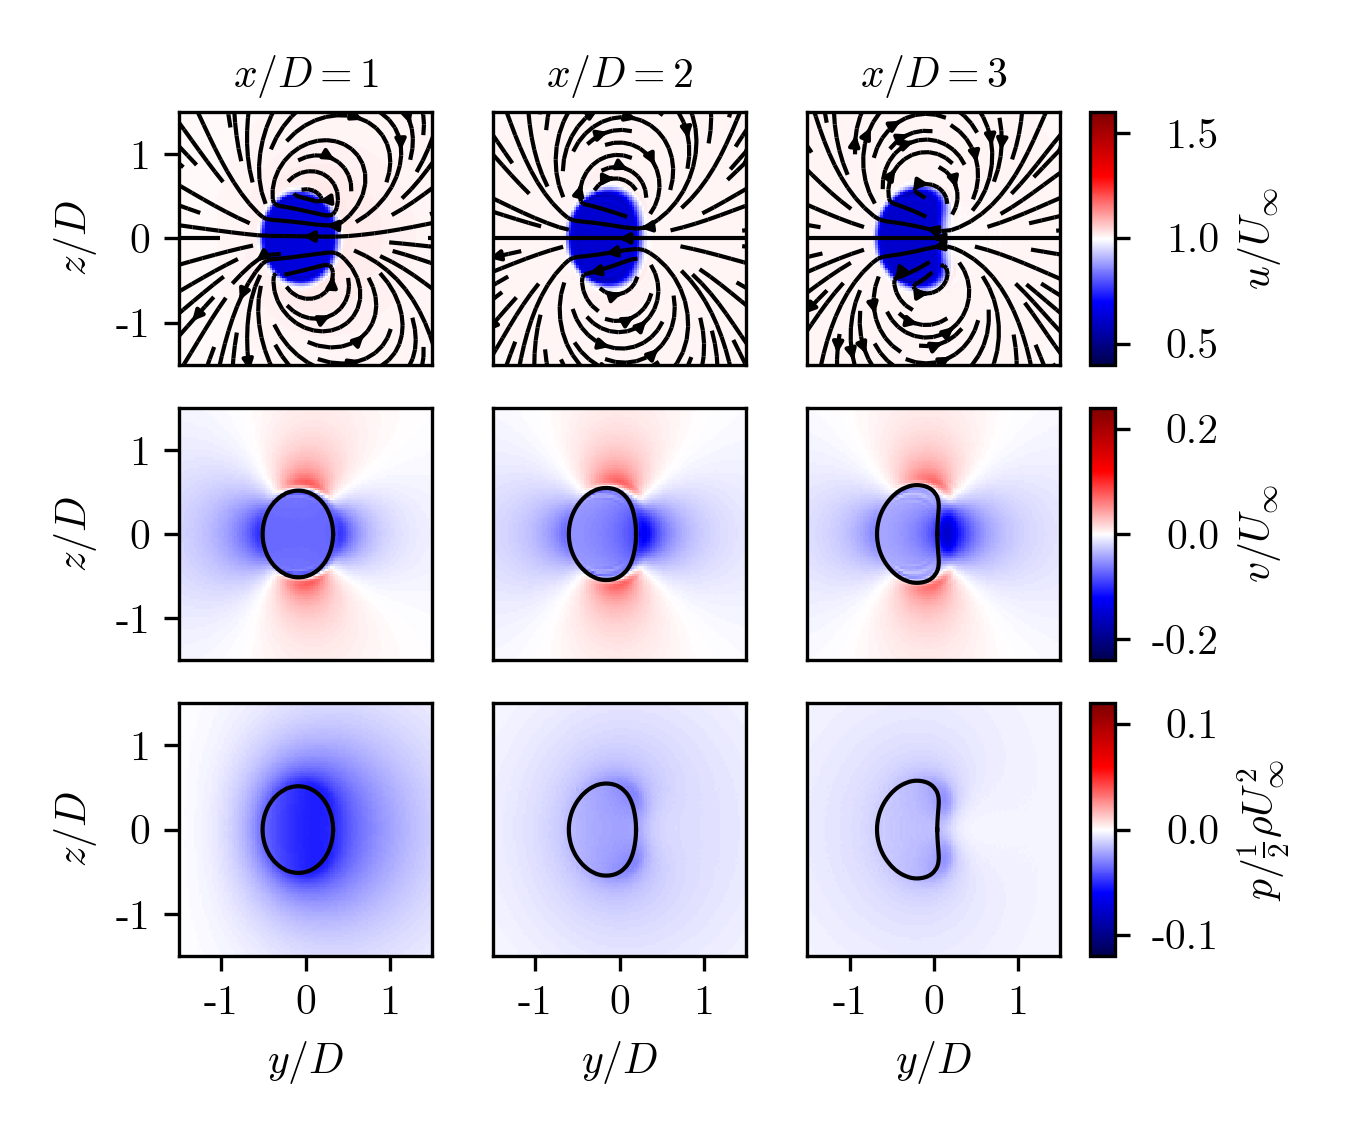
\includegraphics[width=\textwidth]{./fig/yzplane.png}
\caption{\label{fig:yzplane} Simulation results for $C_T' = 1.33$ and yaw angle $\gamma = 30^\circ$ in a domain $L_x/D=11.52$ and   $L_y/D=L_z/D=5.76$.
Shown are color contours of (top) streamwise velocity, (middle) transverse velocity, and (bottom) pressure at downstream locations $x/D = 1$, 2, and 3. Top panels  include streamlines in the $y$-$z$ plane. The transverse velocity and pressure plots show the outline of the wake, defined by the streamtube that passes the rotor at a radius of $r'=0.9R$.}
\end{center}
\end{figure}

In order to provide data to test predictions based on the proposed model above, numerical simulations of flow around a yawed actuator disk under uniform, laminar inflow are carried out using LESGO. A yawed actuator disk of diameter $D$ is placed in a domain of length $L_x=11.52D$ and cross-section size $L_y=L_z=5.76D$ using a total of \mbox{$384 \times 192 \times 192$} grid points. The center of the actuator disk is placed in the center of a $y$-$z$ plane $3.6D$ downstream of the domain inlet.  A uniform inflow velocity $U_\infty$ is applied using a fringe region forcing~\cite{Stevens2014a}.  Molecular viscosity is neglected and the Smagorinsky model is used  for numerical stability with $C_s = 0.16$. Since the flow in the bulk of the near-disk region of interest remains laminar and inviscid and the effect of the subgrid model is confined to the thin shear layer at the boundary of the wake, which is not included in the subsequent analysis, the details of the subgrid modeling are not important for present purposes. The simulations are insensitive to the choice of $C_s$, yielding the same results for $C_s = 0.08$. Various yaw angles $\gamma$ are considered. LESGO uses the local formulation of the thrust force with a local thrust coefficient $C_T'$~\cite{Calaf2010a}. The force is applied using the area fraction function filtered by a three-dimensional Gaussian (see~\eqref{eq:LESGO-Gaussian-kernel}) with a filter width $\sigma_{\mathcal{R}} = 1.5 h / \sqrt{12}$ proportional to the grid size $h = (\Delta x^2 + \Delta y^2 + \Delta z^2)^{1/2}$, where $\Delta x$, $\Delta y$, and $\Delta z$ are the grid spacings.  

Representative results at downstream distances $x/D = 1$, 2, and 3 are shown in  Figure~\ref{fig:yzplane} for $C_T' = 1.33$ and  $\gamma = 30^\circ$. A wake that stays laminar for a large portion of the domain is generated by the actuator disk forcing. At $x/D=1$ near the actuator disk, the wake forms an ellipse with uniform streamwise and transverse velocity components inside of the wake. The transverse component of the force generates the well known counter-rotating vortex pair~\cite{Howland2016a, Bastankhah2016a}, which curls the wake as it moves downstream, shown schematically in Figure~\ref{fig:yawed-actuator-disk-wake}. 

Further simulations are performed at yaw angles $\gamma = 10^\circ$, $20^\circ$, $30^\circ$, and $40^\circ$ and local thrust coefficients $C_T' = 0.8$, $1.0$, and $1.33$.
From these simulations, the spanwise circulation distribution $\Gamma(z)$ is evaluated numerically via integration along rectangular contours running from the inlet of the domain to $x=R$ and spanning the entire width of the domain. The circulation of each shed vortex $\Gamma_0$ is calculated at $x=R$ by averaging the circulation around two rectangular circuits spanning $|y| \le 3R$ and $ |z| \le 3R$. 

We seek to compare the measured results to~\eqref{eq:elliptic-circulation} and~\eqref{eq:gamma0}, for which the disk radius is an important parameter. The footprint of the applied force in the simulations extends slightly from the geometrically prescribed disk dimensions, owing to the use of a filtered area fraction function. To correct for the filtered geometric representation of the disk, the width of an equivalent top-hat filter~\cite{Pope2000a}  $\sqrt{12}\sigma_{\mathcal{R}}=1.5h$ ($h<<R$ is the grid size) is added to the diameter of the disk in~\eqref{eq:gamma0} when applying the inviscid model. The resulting effective radius is $R_*=R+0.75 h$, which leads to the predicted maximum circulation being given by $\Gamma_0 = -(R+0.75 h) \, C_T U_\infty \cos^2\gamma \sin \gamma$. The thrust coefficient is obtained from $C_T = C_T' u_d^2/ (U_\infty \cos \gamma)^2$, where the disk-averaged velocity $u_d$ is measured in the simulations.  As seen in the comparison shown in  Figures~\ref{fig:gamma}(a--b), the predicted circulation distribution and simulation results collapse for all $\gamma$ and $C_T'$ values tested. 

\begin{figure}
\begin{center}
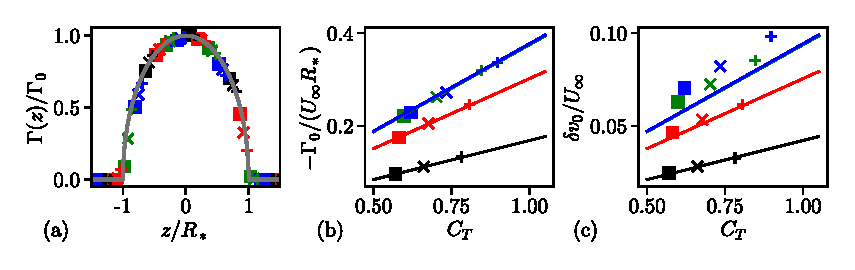
\includegraphics[width=\textwidth]{./fig/gamma.pdf}
\caption{\label{fig:gamma} Comparisons of (a) the measured circulation around the actuator disk (symbols) and the expected distribution from the elliptic lifting line $(1-z^2/R_*^2)^{1/2}$ (grey line), (b) the shed circulation of counter-rotating vortices measured at $x=R$ (symbols) and predicted by lifting line theory (lines), and (c)  the maximum $y$-$z$ planar-averaged transverse velocity measured in the streamtube (symbols) and transverse velocity predicted by lifting line theory (lines). Simulations are conducted with $\gamma = 10^\circ$ (black), $20^\circ$ (red), $30^\circ$ (green), and $40^\circ$ (blue) and $C_T' = 0.8$ ($\blacksquare$), 1.0 ($\times$), and 1.33 ($\bm{+}$). The theoretical values for $\gamma = 30^\circ$ and $40^\circ$ overlap in (b) and (c).}
\end{center}
\end{figure}

Next we compare the transverse velocity magnitude $\delta v_0$ with the model. To measure this value from simulations we take the maximum $y$-$z$ planar-averaged transverse velocity in the wake. The wake is defined as the streamtube passing through the disk at $r' = 0.9R$ to avoid including the thin shear layer near the actuator disk perimeter (results are quite insensitive to this choice). The downstream position of maximum transverse wake velocity occurs very near the disk, at $x \approx R$. Using the thrust coefficient obtained from \mbox{$C_T = C_T' u_d^2/ (U_\infty \cos \gamma)^2$}, we compare $\delta v_0 = \frac{1}{4} C_T U_\infty \cos^2\gamma \sin \gamma$ to simulation measurements in figure \ref{fig:gamma}(c). Again, excellent agreement is observed for various $\gamma$ and $C_T'$ combinations, with a slight underestimate at large $\gamma$. 


\begin{figure}
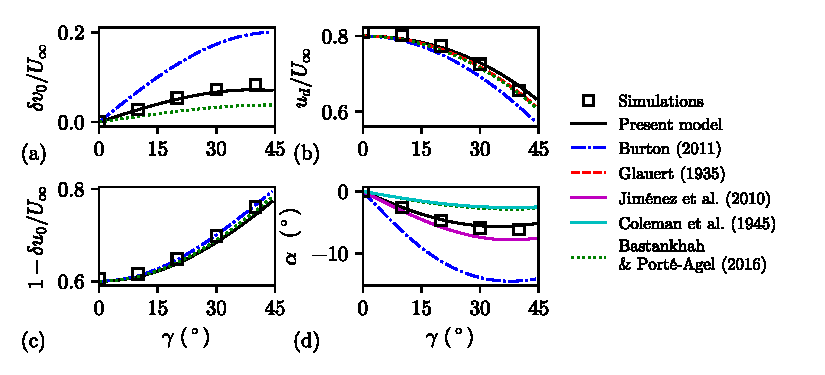
\includegraphics[width=\textwidth]{./fig/steady-uniform-1.pdf}
\caption{\label{fig:steady-uniform}Comparison of (a) transverse velocity $\delta v_0/U_\infty$, (b) disk-averaged velocity $u_d/U_\infty$, (c) streamwise velocity $1 - \delta u_0/U_\infty$,  and  (d) skewness angle $\alpha$ measured in simulations with $C_T' = 1.0$ (squares) with present theory (solid black line) and prior models (other lines).}
\end{figure}

The disk-averaged velocity, streamwise velocity deficit, transverse velocity, and skewness angle of the initial wake obtained from numerical simulations, the present model, and prior models are compared in Figure~\ref{fig:steady-uniform}. The velocity deficit $\delta u_0$ at the end of the inviscid region is obtained from the simulations as the maximum $y$-$z$ planar-averaged streamwise velocity deficit in the wake, which occurs at $x \approx 4D$. The maximum for $\delta u_0$ is further downstream than the maximum for $\delta v_0$ because $\delta u_0$ is strongly affected by streamwise pressure gradients. The transverse velocity prediction~\eqref{eq:deltav0} is expressed using the thrust coefficient $C_T = 16 C_T'/(4 + C_T'\cos^2\gamma)^2$ obtained from the induction factor equation~\eqref{eq:induction_factor}. Predictions for several of the features of the inviscid region are provided by earlier models. Momentum theory~\cite{Burton2011a} provides estimates for all quantities. Glauerts's~\cite{Glauert1926a} equation for the disk-averaged velocity was used by Coleman \textit{et al.}~\cite{Coleman1945a, Burton2011a} to predict the skewness angle of the wake. Bastankhah \& Port\'{e}-Agel~\cite{Bastankhah2016a} recently used momentum conservation, the Bernoulli equation, and approximations to Glauert's and Coleman's equations to predict the streamwise and transverse velocities behind the disk. Jimenez \textit{et al.}~\cite{Jimenez2010a} used momentum balance arguments to predict the initial wake deflection angle. 

Figure~\ref{fig:steady-uniform} shows that the present inviscid region model accurately predicts the quantities measured in simulations. In contrast, other models show significant disagreement in the skewness angle and transverse velocities. Momentum theory and Jim\'{e}nez's~\cite{Jimenez2010a} equation overestimate the skewness angle and transverse velocity magnitudes. The skewness angle magnitude predicted by Coleman~\cite{Coleman1945a}, and by extension the transverse velocity magnitude predicted by Bastankhah \& Port\'{e}-Agel~\cite{Bastankhah2016a}, are approximately half as large as those obtained in the simulations. While Coleman's~\cite{Coleman1945a} prediction may improve downstream as the wake is transformed by the counter-rotating vortex pair, this skewed elliptic vortex cylinder argument becomes less valid as a result of the curling. 

\section{Wake model for yawed turbines}
\label{sec:yaw-wakemodel}
An important application of the inviscid region theory described in the prior section is to determine an initial condition for models of the turbulent wake behind yawed turbines. We demonstrate the utility of the proposed inviscid region model by applying the predictions to the wake model of Section~\ref{sec:dynwake-wakemodel}.  Retaining the $u$ and $v$ components of the model, the velocity deficit source strengths, $S_1  = U_\infty \delta u_0$ and $S_2 = U_\infty \delta v_0$, are based on the inviscid model, where $\delta u_0$ and  $\delta v_0$ are given by~\eqref{eq:sys2} and \eqref{eq:deltav0}. This approach provides a smooth increase of the streamwise and transverse velocity deficits from zero upstream of the rotor to the desired `wake initial condition' downstream of the rotor region. 

The average streamwise velocity deficit $\delta u(x,t)$ is distributed using a Gaussian profile~\cite{Bastankhah2014a, Bastankhah2016a}, which along $z=0$ reads
\begin{equation}
\label{eq:u_model}
u(x,y,t) = U_\infty - \delta u(x,t) \, \frac{D^2}{8 \sigma_0^2} \,\exp \left(-  \frac{(y-y_c(x,t))^2}{2\sigma^2(x)} \right), 
\end{equation}
where the width of the Gaussian $\sigma(x) = \sigma_0 d_w(x)$ is proportional to the effective normalized wake diameter with a proportionality constant $\sigma_0$. The velocity deficits are found by integrating~\eqref{eq:preliminary_deficit}, and the wake centerline $y_c(x,t)$ is found by integrating the transverse velocity according to
\begin{equation}
\frac{\partial y_c}{\partial t} + U_\infty \frac{\partial y_c}{\partial x} = -\delta v(x,t).
\end{equation}
in the positive $x$ direction subject to $y_c = 0$ far upstream of the turbine. The negative sign occurs because $\delta v(x,t)$ is a deficit in our sign convention. 
Equation~\eqref{eq:u_model} is consistent with~\eqref{eq:area_velocity}; i.e. $\int_{0}^\infty (U_\infty - u) 2\pi \xi d\xi = A(x)\delta u(x,t)$, where the distance $\xi = y-y_c(x,t)$ is measured from the wake centerline at $y_c(x,t)$.
 
\begin{figure}[h!]
\begin{center}
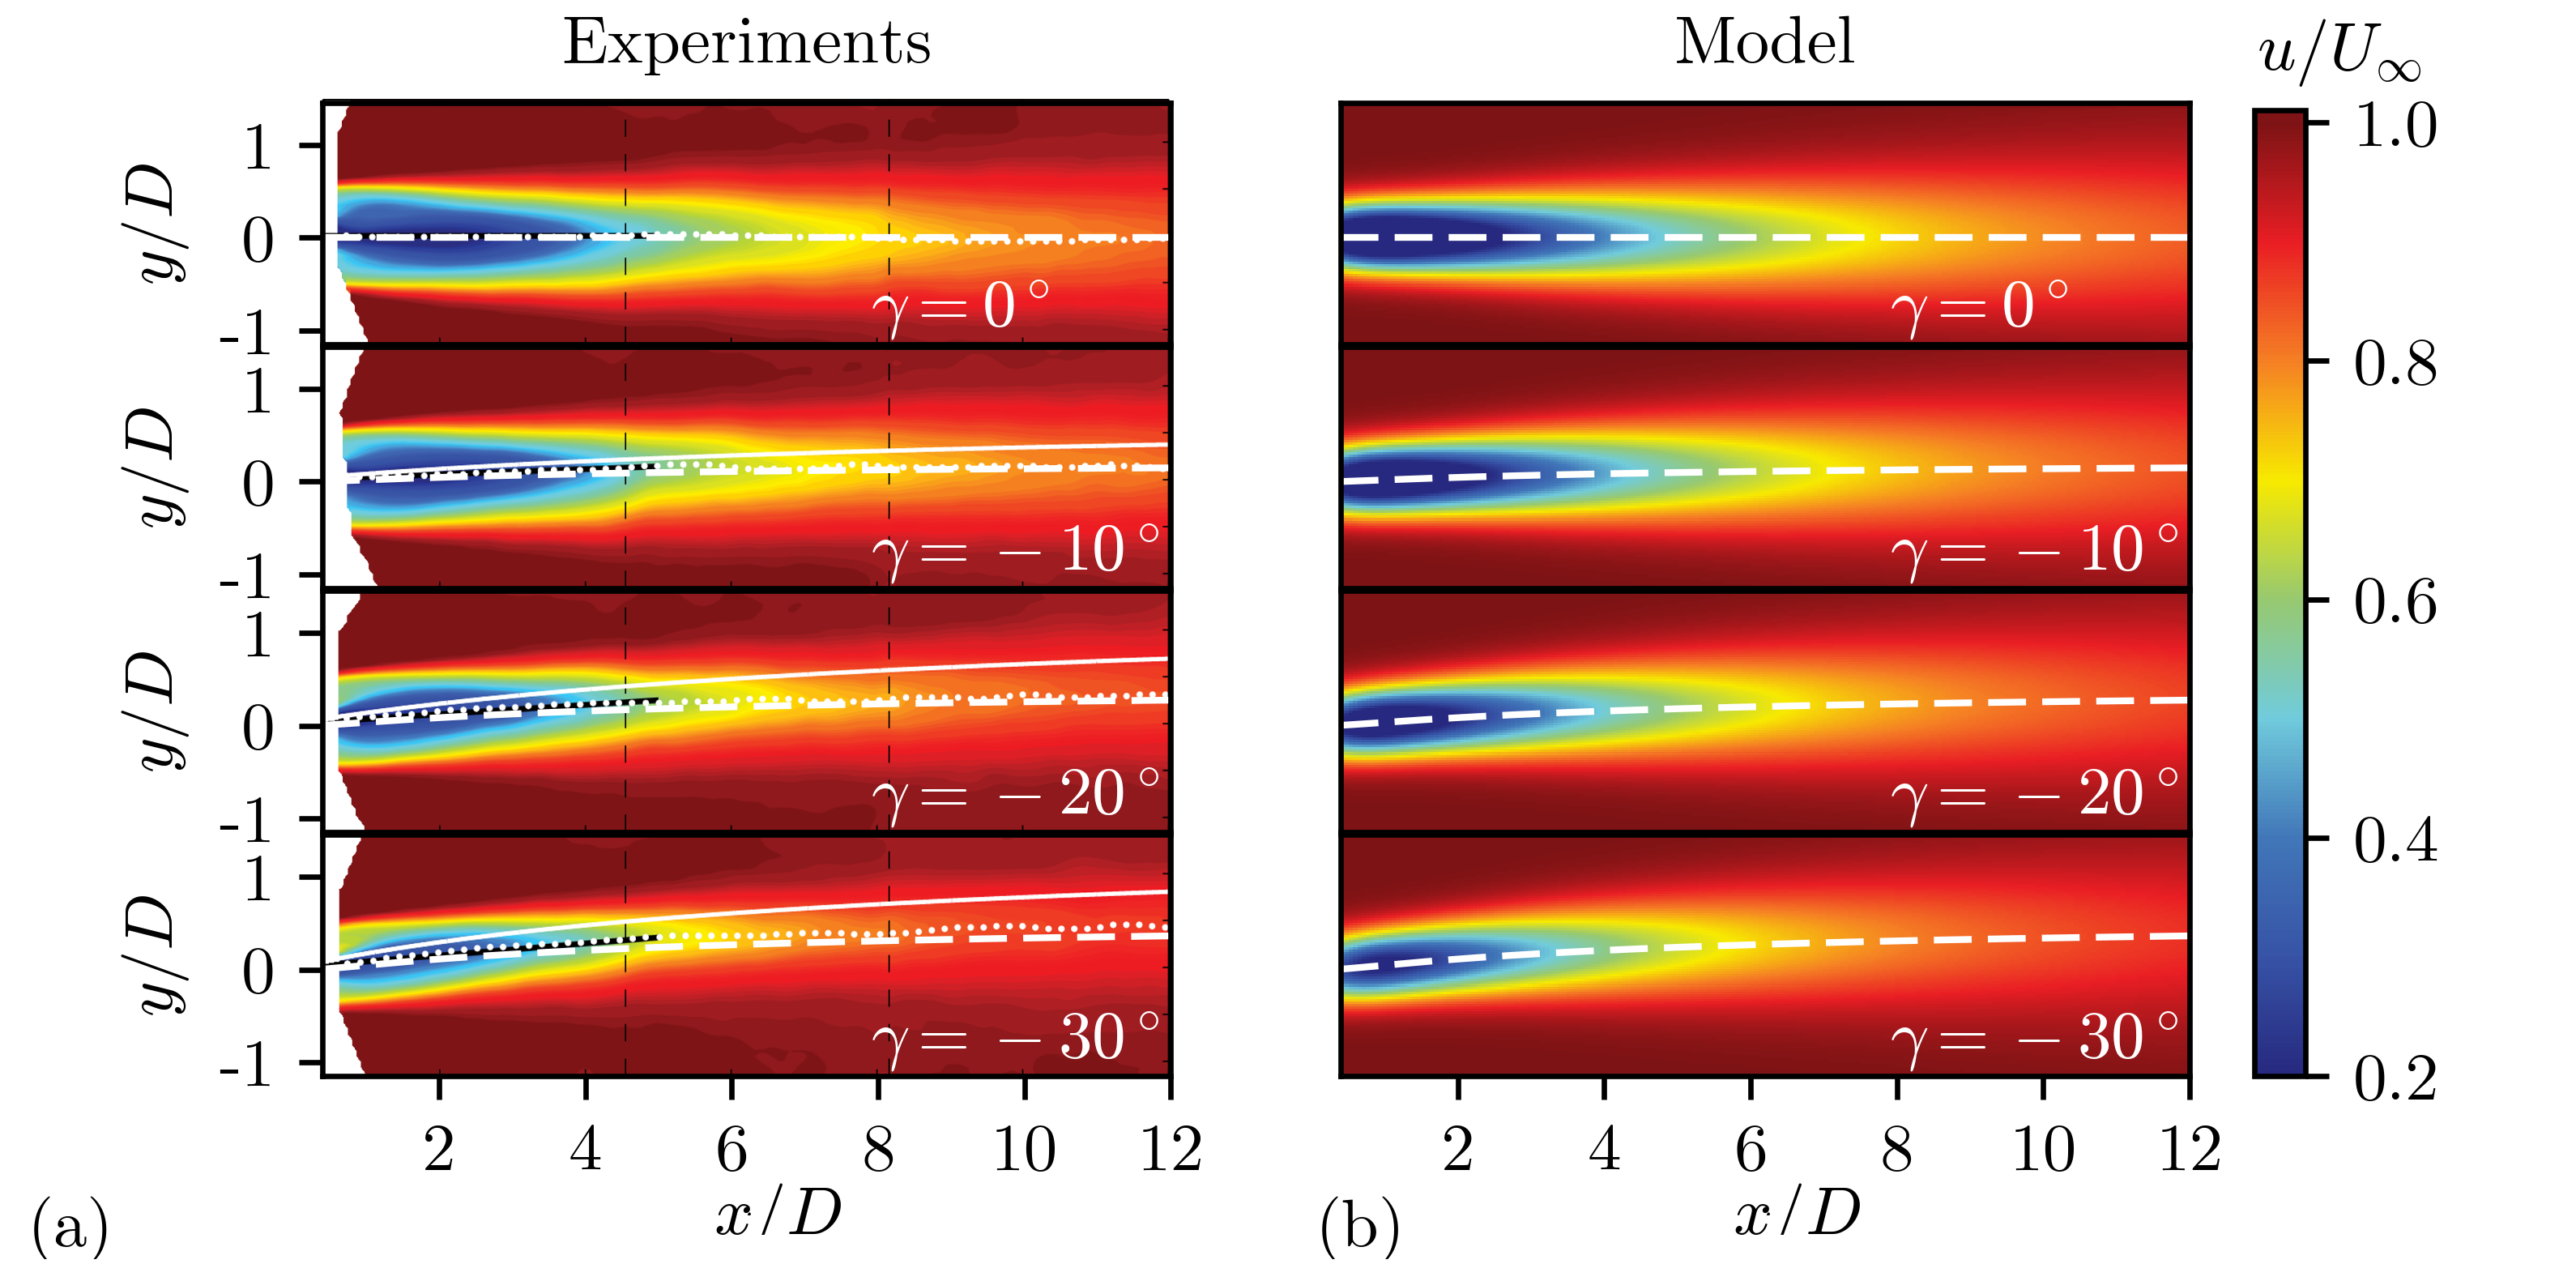
\includegraphics[width=\textwidth]{./fig/bastankhah_comparison_overlay.png}
\caption{\label{fig:far_wake} Hub-height color contour plots of streamwise velocity as (a) measured in experiments~\cite{Bastankhah2016a} and (b) predicted using the proposed model. 
Measured centerlines of the wake (dotted) are compared to the model of~\cite{Jimenez2010a} (solid) and the present model (dashed).  Experimental data in (a) adapted with permission from figure 3 of Bastankhah and Port\'{e}-Agel\cite{Bastankhah2016a}.}
\end{center}
\end{figure}

While this model includes possible time-dependence (e.g. the turbine's local thrust coefficient and yaw angle could change over time), in this chapter, we focus solely on the steady-state solution and compare it to the wind tunnel experiments of Bastankhah and Port\'{e}-Agel~\cite{Bastankhah2016a} that were performed under steady conditions. The steady-state version of this wake model, where time derivatives vanish and the solution found by integrating in $x$,
\begin{align}
\delta u(x) &= \frac{\delta u_0}{d_w^2(x)} \frac{1}{2}\left[1 + \mathrm{erf}\left(\frac{x}{\Delta_w \sqrt{2}}\right)\right]\\
\delta v(x) &= \frac{\delta v_0}{d_w^2(x)} \frac{1}{2}\left[1 + \mathrm{erf}\left(\frac{x}{\Delta_w \sqrt{2}}\right)\right]\\
y_c(x) &= \int_{-\infty}^x \frac{-\delta v(x')}{U_\infty} dx'
\end{align}
is compared to wind tunnel experiments by Bastankhah \&Port'{e}-Agel~\cite{Bastankhah2016a}. We use the experimental data for the un-yawed \mbox{($\gamma = 0^\circ$)} case to fit the two required  parameters $k_w$ and $\sigma_0$, obtaining very reasonable values $k_w=0.0834$ and  $\sigma_0 /D = 0.235$. 
The measured thrust coefficients of the rotating turbine (depending on the yaw angle, as reported by Bastankhah and Port\'{e}-Agel\cite{Bastankhah2016a}) are used to set the initial velocity deficits $\delta u_0$ and $\delta v_0$ in the model. Figure~\ref{fig:far_wake} compares the streamwise velocity deficit at hub height for $\gamma = 0^\circ$, $-10^\circ$, $-20^\circ$, and $-30^\circ$. The centerlines of the measurements are compared to the present model and the model of Jimenez \textit{et al.}~\cite{Jimenez2010a}. The proposed model is found to be in excellent agreement with the experiments, particularly the estimate of the centerline of the wake.  

\section{Conclusions}
\label{sec:yaw-conclusions}
Previous models for the inviscid region near a yawed actuator disk have generated conflicting predictions for the initial transverse velocity and skewness angle of the wake that fail to match actuator disk simulations. Accurate models for this inviscid region are vital for developing useful wake models for engineering design and control applications. In this chapter, we derive a new model of the flow in the inviscid region near the disk. It treats the yawed actuator disk as an elliptically loaded lifting line and uses Prandtl's lifing line theory to determine the initial transverse velocity deficit and magnitude of the counter-rotating vortex pair shed from the yawed actuator disk. Momentum conservation and Bernoulli's equation are then applied to determine the disk-averaged velocity and streamwise velocity deficit. The predictions are found to agree with numerical simulations and accurately estimating the initial transverse velocity.  We use the inviscid region predictions as initial conditions for a simple model of the flow field behind a yawed turbine and compare to experimental data. 
The newly proposed combined model for the inviscid and wake regions is remarkable for its simplicity and success at reproducing a variety of observations.

